\chapter{Event Reconstruction}\label{chap:reco}
	Before any physics analysis can be performed on the raw data from the ATLAS detector and MC simulations both raw datasets go through a reconstruction software suite called Athena. Various algorithms are employed to identify energy deposits as particles based on shower shapes, tracker hits, calculated charge to mass ratios, etc. Figure \ref{fig:ATLAS-XSec} shows the signatures of various particles within the ATLAS detector. 

	\begin{figure}[!ht]
	\centering
	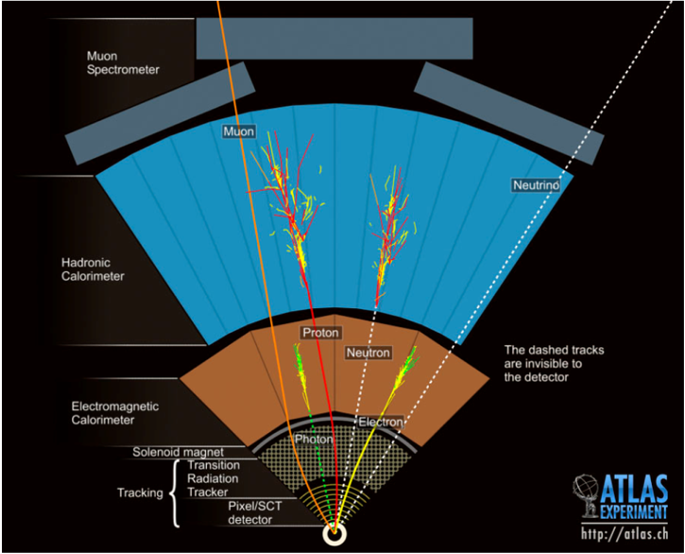
\includegraphics[width=.65\textwidth,keepaspectratio=true]{chapters/chapter3_experiment/images/ATLASCrossSectionDiagram.png}
	\caption{ Cross section view of the ATLAS detector with subdetectors labeled. Various types of particles radial trajectories are shown.}
	\label{fig:ATLAS-XSec}
	\end{figure}

	The following sections detail the identification processes of muons, electrons, photons, jets, $\tau$ leptons, and a calculated quantity called missing transverse energy $(\Etm)$. These reconstructed physics objects are the inputs to the majority of physics analyses.

	\section{Tracks}
	Tracks are fits connected three dimensional space-points in the ID. These space-points are created from clusters of hits in the ID. A set of three space-points are combined into one track seed, then fed into three methods in the ATLAS detector: inside-out,  outside-in, and TRT-standalone. The inside-out method creates tracks by starting with a seed hit in the pixel detector, then SCT hits are added, finally the track is extrapolated out into the TRT. This method creates tracks of particles that are mostly produced in the hard \pp interaction and has a requirement of $\pt>400$ MeV. On the other-hand the outside-in method starts with track segments in the TRT and extrapolates towards the beamline using silicon that were not used in the inside-out method. Outside-in tracking typically reconstructs secondary vertices from particles that have long enough lifetimes to decay while inside the ID, including b quarks and $\tau$ leptons. Lastly, TRT-standalone tracks are made only from seeds within the TRT and are not extrapolated to the silicon subdetectors  \cite{ATLAS-perf-run2}. The reconstructed tracks are used in the identification of various types of particles.

	% Reconstructed tracks are made at two working points (WPs) to give analyzers a variety of track fits to best fit the analysis' needs
	% \begin{multicols}{2}
	% \begin{itemize}
	% 	\item Loose
	% 	\begin{itemize}
	% 		\item $p_{T} > 400$ MeV
	% 		\item $|\eta|<2.5$
	% 		\item $\geq 7$ silicon hits
	% 		\item $\leq 1$ shared modules
	% 		\item $\leq 2$ silicon holes
	% 		\item $\leq 1$ pixel holes
	% 	\end{itemize}
	% 	\item Tight
	% 	\begin{itemize}
	% 		\item if $|\eta|<1.65$
	% 		\begin{itemize}
	% 			\item $\geq 9$ silicon hits
	% 		\end{itemize}
	% 		\item if $|\eta| > 1.65$
	% 		\begin{itemize}
	% 			\item $\geq 11$ silicon hits
	% 			\item 1 hit on 2 innermost pixel layers
	% 			\item 0 pixel holes
	% 		\end{itemize}
	% 	\end{itemize}
	% \end{itemize}	

	% \end{multicols}

	\section{Topological Clusters}
	A topocluster is defined as a cluster of topologically connected calorimeter cell signals. Topological clusters in the ATLAS detector's calorimeters are vital to the identification of hadronic final states, meaning jets (Section \ref{sec:reco-jets}), isolated hadrons, and hadronically decaying $\tau$ leptons (Section \ref{ssec:reco-tau}). Topoclusters are also included in the calculation of missing transverse energy discussed in Section \ref{sec:reco-etmiss}, as they represent the direction and energy of softer particles in a collision event. 

	A topocluster is created via a growing volume algorithm that operates based on a set of three thresholds. These thresholds are defined using the calorimeter cell significance $\xi_{cell}$ \cite{topocluster-perf}. 
	\begin{equation}
	\xi_{cell} = \frac{E_{cell}}{\sigma_{noise, cell}}
	\end{equation}
	Where $E_{cell}$ is the energy in the calorimeter cell and $\sigma_{noise, cell}$ is the average expected noise of a given calorimeter cell. An in-depth review of how the $\sigma_{noise, cell}$ value is calculated for TileCal is given in \ref{app:Tile-DQ}. A topocluster starts with a seed cell that has a significance greater than the seed threshold S. From the seed cell, all three-dimensionally neighboring cells with a significance greater than the growth threshold N are added to the topocluster. This is done repeatedly until there are no more neighboring cells that pass the requirement $|\xi_{cell}|>N$. If a neighboring cell also passes the $|\xi_{cell}|>S$ threshold, then the topocluster corresponding to the neighbor cell is merged into the original topocluster. Finally, a last layer of the topocluster is added from all neighboring cells passing a threshold of $|\xi_{cell}|>P$. In the ATLAS experiment, the threshold values are set at $(S,N,P) = (4,2,0)$.

	\section{Muon Identification}\label{sec:reco-muon}
	Muons are identified using a combination of information from the ID and the MS. Within the ID, muons leave tracks identical to any other charged particle; however, in the MS tracks are identified within the MDTs through a straight-line fit in a single layer and by doing a combinatorial search of CSC hits in the $\eta-\phi$ plane. \cite{muon-id} Muons are identified through five strategies, each using the information from the ID, MS, and calorimeter (in one case).
	\begin{itemize}
		\item Combined (CB): Match ID and MS tracks. Perform a combined track fit on ID and MS hits. Takes into account energy loss in calorimeters
		\item Inside-Out (IO): Extrapolate ID tracks, look for at least three loosely aligned MS hits. Calorimeter energy loss is accounted for.
		\item Muon Spectrometer Extrapolated (ME): Extrapolate MS tracks back to the beamline. No ID hits are taken into account.
		\item Segmented-Tagged (ST): Extrapolate ID tracks and match to MS segments with tight angular requirement. Muon parameters are taken directly from the ID.
		\item Calorimeter-Tagged (CT): Extrapolate ID tracks into the calorimeters. Look for energy deposits consistent with minimum ionizing particles. Tag as muon, take parameters from ID.
	\end{itemize}
	All muon identification strategies have a transverse momentum cut on ID tracks of $\pt^{track}> 2$ GeV, except for CT, which has a cut of $\pt^{track} > 5$ GeV.
	
	Reconstructed muons are divided into three WPs to allow analyzers a choice of purity, efficiency, and background rejection. 
	\begin{itemize}
		\item Loose: Optimized for reconstruction of $H\rightarrow4\mu$. Lowest purity and highest efficiency.
		\item Medium: Efficiency and purity are suitable for a wide range of analyses with small systematic uncertainties.
		\item Tight: High purity, slightly lower efficiency than medium WP. Significantly higher background rejection.
	\end{itemize}


	\section{e $\gamma$ Identification}\label{sec:reco-egamma}
	\cite{electron-perf}

	\section{Jet Clustering}\label{sec:reco-jets}

		\subsection{\bjet Tagging}\label{ssec:flavor-tagging}

	\section{$\tau$ Identification}\label{ssec:reco-tau}


	\section{\Etm}\label{sec:reco-etmiss}
	\cite{met-perf}

	\section{Particle Flow}\label{sec:pflow}
	\cite{pflow}

	\begin{figure}[!ht]
	\centering
	
\includegraphics[width=\textwidth,keepaspectratio=true]{chapters/chapter5_eventreconnstruction/images/pflow_flow_chart.png}
	\caption{\label{fig:pflow} A flow chart of how the particle flow algorithm proceeds, starting with track selection and continuing until the energy associated with the selected tracks has been removed from the calorimeter. At the end, charged particles, topoclusters which have not been modified by the algorithm, and remnants of topoclusters which have had part of their energy removed remain. \cite{pflow}}
	\end{figure}